\chapter{Solution}

\section{Eclipse Sirius}
Les débuts du développement d’un modèle pour Eclipse Sirius fut très fastidieux. Après avoir passé un bout de temps sur le tutoriel présent sur le site je me suis confronté a un manque d’autres exemples me permettant de vraiment prendre en main Sirius. Le manque d'informations à été comblé par l'équipe en charge du développement de Sirius. Cependant les démarches pour disposer d'une formation dans leur locaux à Nantes à pris trop de temps pour différentes raisons et nous avons du mettre de coté cette partie de la solution.

\section{Application Web}
Pour la partie sur l'application Web, ma premier démarche a été de trouver une bibliothèque JavaScript capable de générer un graphe orienté cyclique. Google m’a diriger vers une question similaire sur stackoverflow. J’ai bénéficié d'un comparatif complet des existants, avec pour chacun leurs avantages et inconvénients. Mon choix s’est porté sur cytoscape.js. Cytoscape avait l’avantage de réaliser rapidement un graphe correspondant à mes besoin depuis un fichier JSON. Il offre de plus une intégration avec jQuery et/ou Angular pour la manipulation du DOM. Il est sous licence GPL ce qui faisait partie des impératifs du projet. Enfin Cytoscape propose par défaut une dizaine de layouts utilisables pour explorer le graphe de différentes manière.
\clearpage
\section{Développement de l'outil}

\subsection{Tableau JSON}
La première chose pour pouvoir exploiter un affichage du graphe des champs du formulaire avec Cytoscape est de générer un fichier Json. Le fichier contenant une liste d'objet représentant soit un noeud soit une arête. 
\begin{lstlisting}
      { data: { id: 'foo' }, group: "nodes" },
      { data: { id: 'bar' }, group: "nodes" },
      { data: { id: 'baz', source: 'foo', target: 'bar' }, group: "edges" }
\end{lstlisting}
En se servant de la bibliothèque de Google Gson qui permet de transformer un objet Java en objet Javascript, il a été necessaire de créer des classes correspondant aux critères de Cytoscape. Il a fallu par la suite générer un fichier pour chaque formulaire au format Json contenant chaque champs avec les données qui lui sont propres et les dépendances sous formes d'arètes.

\subsection{Génération de code}
Au seins du code Java il à fallu utiliser l'API Réflection pour pouvoir utiliser les informations sur les champs des formulaires. Ainsi à l'aide de ce mécanisme il m'a été possible de calculer les dépendances entre les champs, les types de champs utilisés ainsi que d'autres informations qui seront mises à jour à chaque compilation de l'application par Maven.

\begin{lstlisting}[caption=Introspection du JAR]
    private Collection<Object> getFactories(String className, ClassLoader classLoader) throws Exception {
        final List<Object> factories = new ArrayList<>();
        final Class<?> clazz = Class.forName(className, true, classLoader);
        for (Class<?> enumType : new Reflections("net.courtanet", classLoader).getSubTypesOf(clazz)) {
            if (Modifier.isPrivate(enumType.getModifiers()))
                continue;
            if (!enumType.getSimpleName().startsWith("BundleField"))
                continue;
            factories.add(enumType.newInstance());
        }
        return factories;
    }
\end{lstlisting}
\begin{multicols}{2}
\begin{lstlisting}[caption=Exemple de fichier JSON généré]
[
  {
    "data": {
      "label": "SCR_CLAIM",
      "id": "SCR_CLAIM",
      "type": "SCREEN"
    },
    "group": "nodes"
  },
  {
    "data": {
      "label": "Votre assurance",
      "id": "BLK_ASSURANCE",
      "parent": "SCR_CLAIM",
      "type": "BLOCK"
    },
    "group": "nodes"
  },
  {
    "data": {
      "label": "CLAIM_DATE",
      "help": "no_help",
      "tip": "no_tip",
      "id": "CLAIM_DATE",
      "parent": "BLK_ASSURANCE",
      "type": "VALUE_OBJECT"
    },
    "group": "nodes"
  },
  {
    "data": {
      "id": "ADRESSE_LIVRAISON_DIF",
      "source": "ADRESSE_LIV_DIF",
      "target": "LIVRAISON_ADR1"
    },
    "group": "edges"
  },
\end{lstlisting}

\end{multicols}
\subsection{Génération du graphe}
La logique par la suite était de servir les fichiers Json de façon asynchrone à la demande d'affichage du graphe d'un des formulaire de LesFurets.com. Pour cela la solution vers laquelle je me suis tourner était la manipulation du DOM à l'aide de AngularJS. Cytoscape permet à l'aide de closure de modifier le graph qu'en cas de modifications défini dans le "controller" AngularJS. 
\vspace{0.2in}
\begin{figure}[!ht]
\center

\includegraphics[width=15cm]{outil/buttons-tunnels.png}
\caption{Choix du formulaire}
\end{figure}
Ainsi à chaque demande du graphe d'un formulaire à l'aide d'un des boutons de l'interface on demande si le tableau JSON existe. Si il existe on trace le graphe sinon on fait un appel au serveur, une fois le fichier reçu on lance le calcule du graphe. Si il y a une attente, on affichera un élégant loader invitant l'utilisateur à prendre son mal en patience. 

\subsection{Zoomer, déplacer les éléments, se déplacer}
Une fois le graphe affiché il est apparu essentiel de pouvoir laisser l’utilisateur zoomer, se déplacer dans le graphe et déplacer les éléments du graphe. A l'aide de la documentation de l'API et aux fonctionnalités permises par la balise canvas de HTML5, j'ai pu définir des fonctions de glisser déposer pour déplacer les éléments ainsi que pour déplacer tout le graphe. Enfin pour les fonctions de zoom j'ai défini le graphe en position relative et j'ai utilisé l'évènement onscroll.

\subsection{Layout du graphe}
Cytoscape dispose d'un système pour permettre aux développeur de définir leur layout. Un layout n'étant qu'un ensemble de règles définies pour afficher les noeuds et arêtes sous forme de graphe.
\begin{lstlisting}[caption=Exemple d'un layout traçant le graphe sous forme de cercle]
var layoutCircle = {
  name: 'circle',
  fit: true, // whether to fit the viewport to the graph
  padding: 30, // the padding on fit
  avoidOverlap: true, 
  radius: undefined, 
  startAngle: 3/2 * Math.PI, 
  counterclockwise: false, 
};
\end{lstlisting}
Enfin on laissera la possibilité à l'utilisateur de choisir le layout dont il aura besoin.
\begin{figure}[!h]
\centering
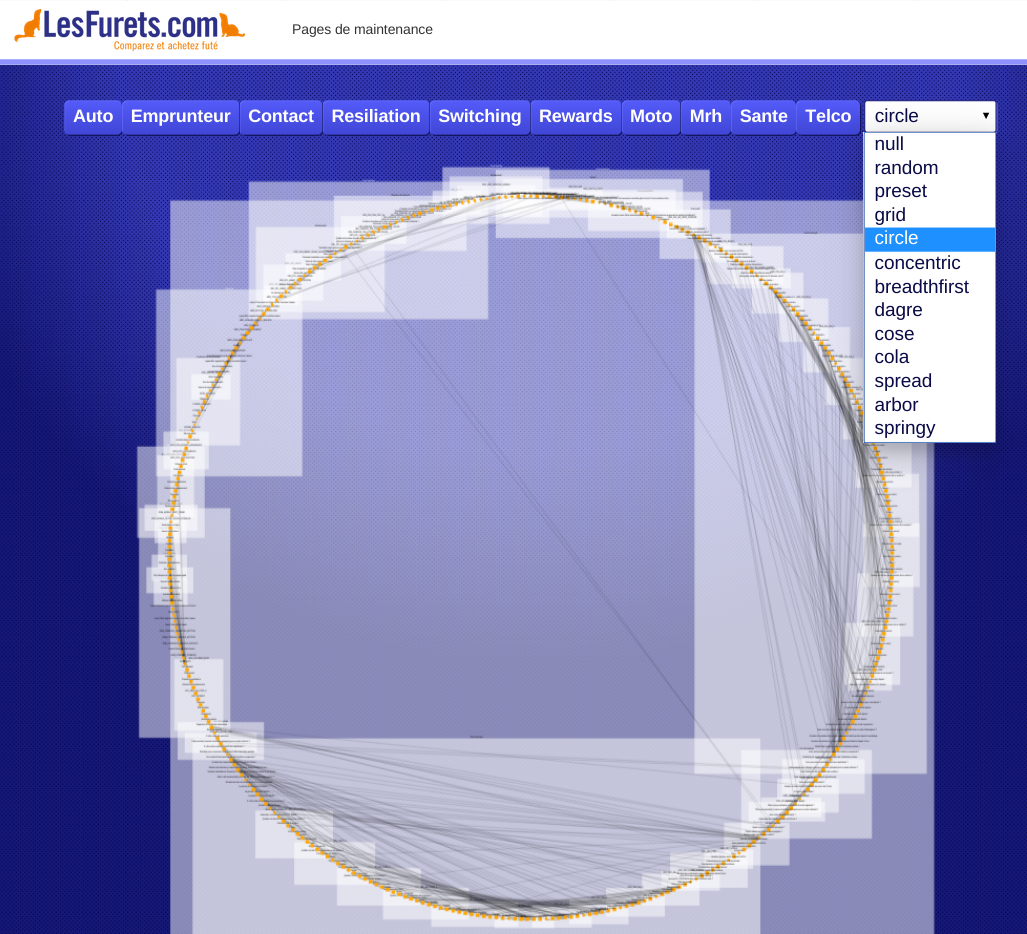
\includegraphics[height=7cm]{outil/layout-circle.png}
\caption{Graphe tracé avec un layout "circle"}
\end{figure}

\subsection{Layout WireFrame}
On proposera un layout "wireframe" qui permettra d'afficher le graphe sous une forme similaire au formulaire proposé sur le site. C'est a dire que tous les écrans sont disposés à la suite les uns des autres et que sont disposé à l'intérieur, verticalement, les champs du formulaire. 
Pour cela il m'a fallut réaliser deux opérations non triviales : 
\begin{itemize}
\item 
Modifier la structure du JSON pour inclure une donnée permettant de définir l'ordre des des écrans, blocs, groupes, champs du formulaire.
\item
Écrire une fonction dans mon code JavaScript permettant de positionner horizontalement et verticalement les éléments.
\end{itemize}
\vspace{0.5in}
\begin{figure}[!h]
\centering
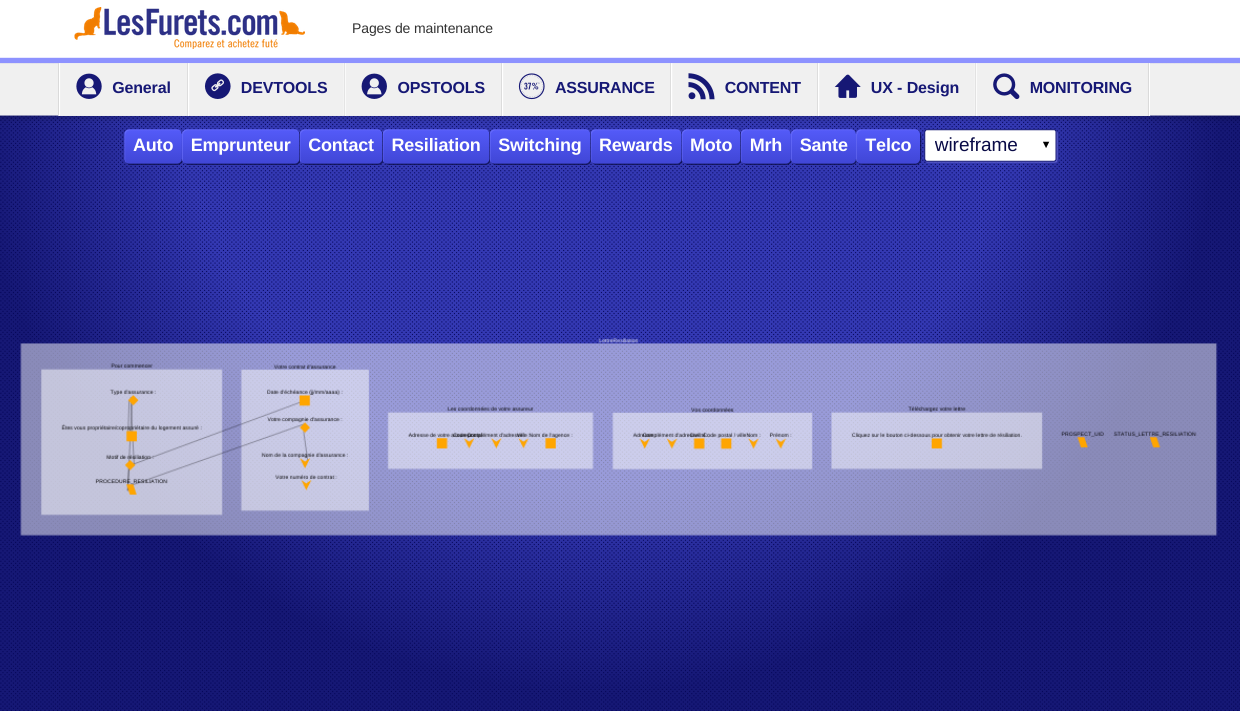
\includegraphics[width=16cm]{outil/layout-wireframe.png}
\caption{Formulaire Résiliation avec le Layout Wireframe}
\end{figure}
\clearpage
\subsection{Layout DAG}
On proposera aussi un layout "dag" qui affichera le graphe avec en évidence les cycles et les dépendances plus fortes. Pour cela on calculera les dépendances entres les champs. On calculera le score de chaque élément en fonction de son nombre total d'arêtes liées à un élément parent diffèrent, que ce soit un écran, un bloc ou un groupe. Enfin on disposera au plus proche les éléments en fonction des deux éléments contenus ayant les plus grands scores. Ce layout sera intéressant pour des formulaires avec un grand nombre d'éléments pour visualiser les dépendances entres les éléments du formulaire.
\vspace{0.5in}
\begin{figure}[!h]
\centering
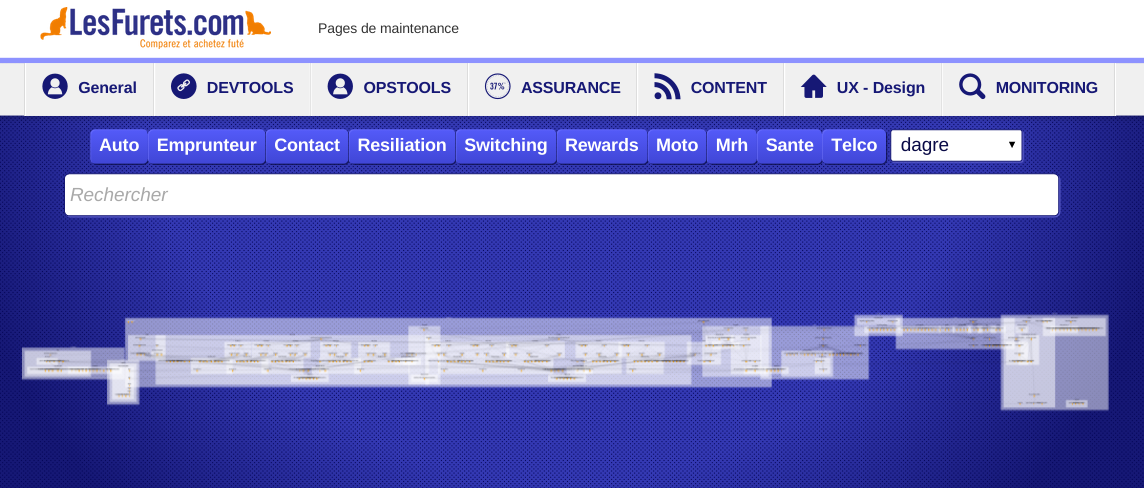
\includegraphics[width=15cm]{outil/layout-dagre.png}
\caption{Formulaire Assurance Auto avec le Layout DAG}
\end{figure}
\begin{figure}[!h]
\centering
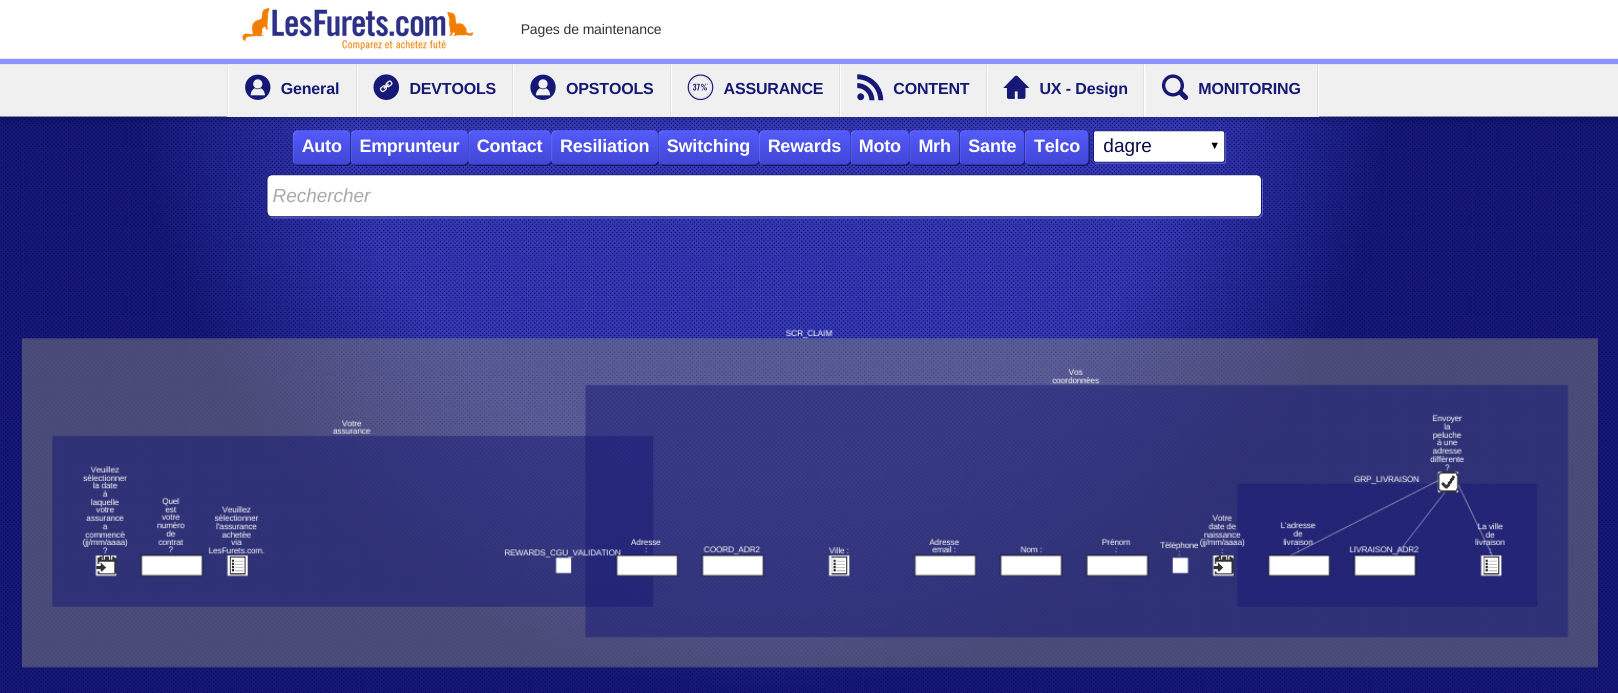
\includegraphics[width=15cm]{outil/layout-dag-2.png}
\caption{Formulaire Rewards avec le Layout DAG}
\end{figure}
\clearpage
\subsection{Recherche d’un champs et autocompletion}
Une fois le graphe affichant tous les champs du formulaire il nous a paru nécessaire de pouvoir rechercher un champs et de pouvoir zoomer sur celui-ci. Ma première approche était d'écrire une fonction capable de zoomer sur un élément du graphe depuis le code. Une fois celle-ci implémentée, il à été facile de zoomer sur le champs et par la suite de zoomer sur son élément parent direct.
\vspace{0.5in}
\begin{figure}[!h]
\centering
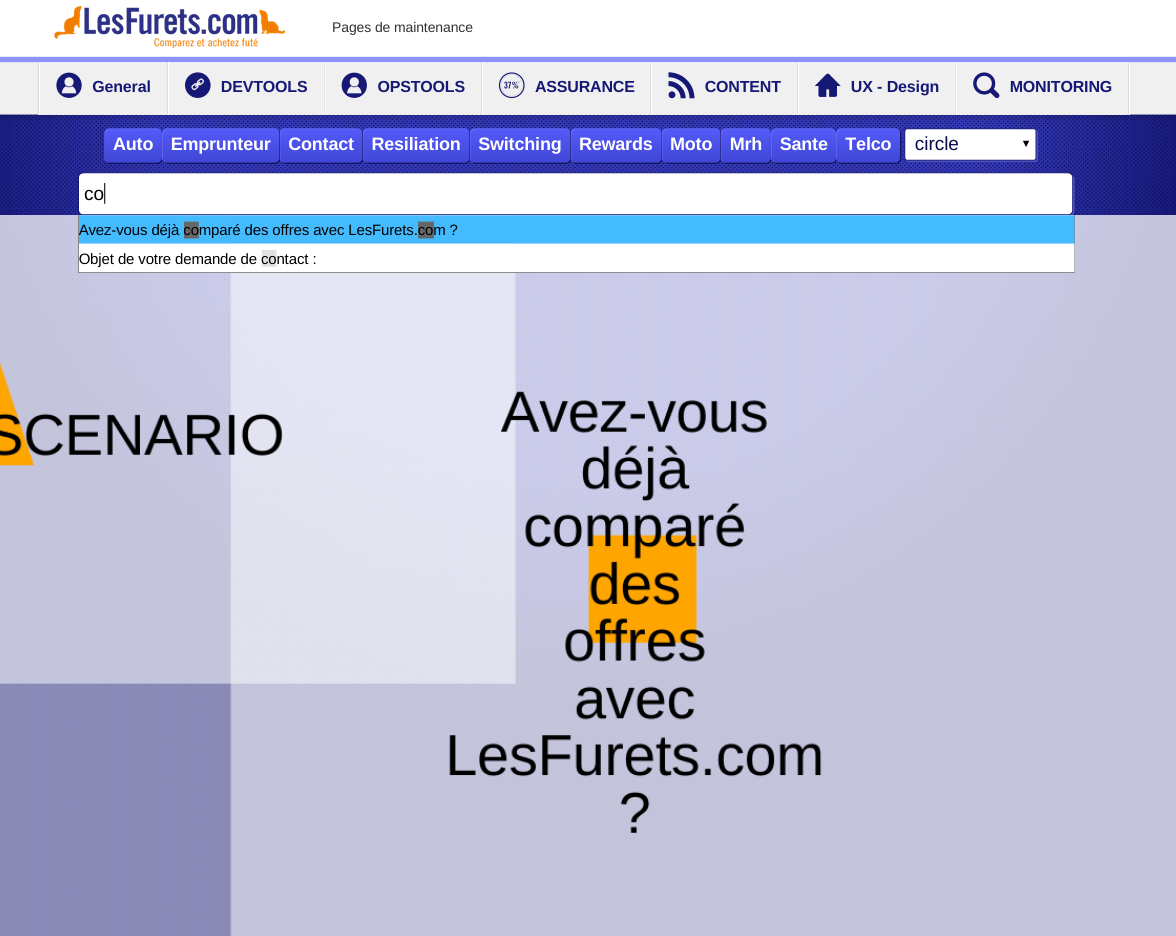
\includegraphics[height=4cm]{outil/feature-search.png}
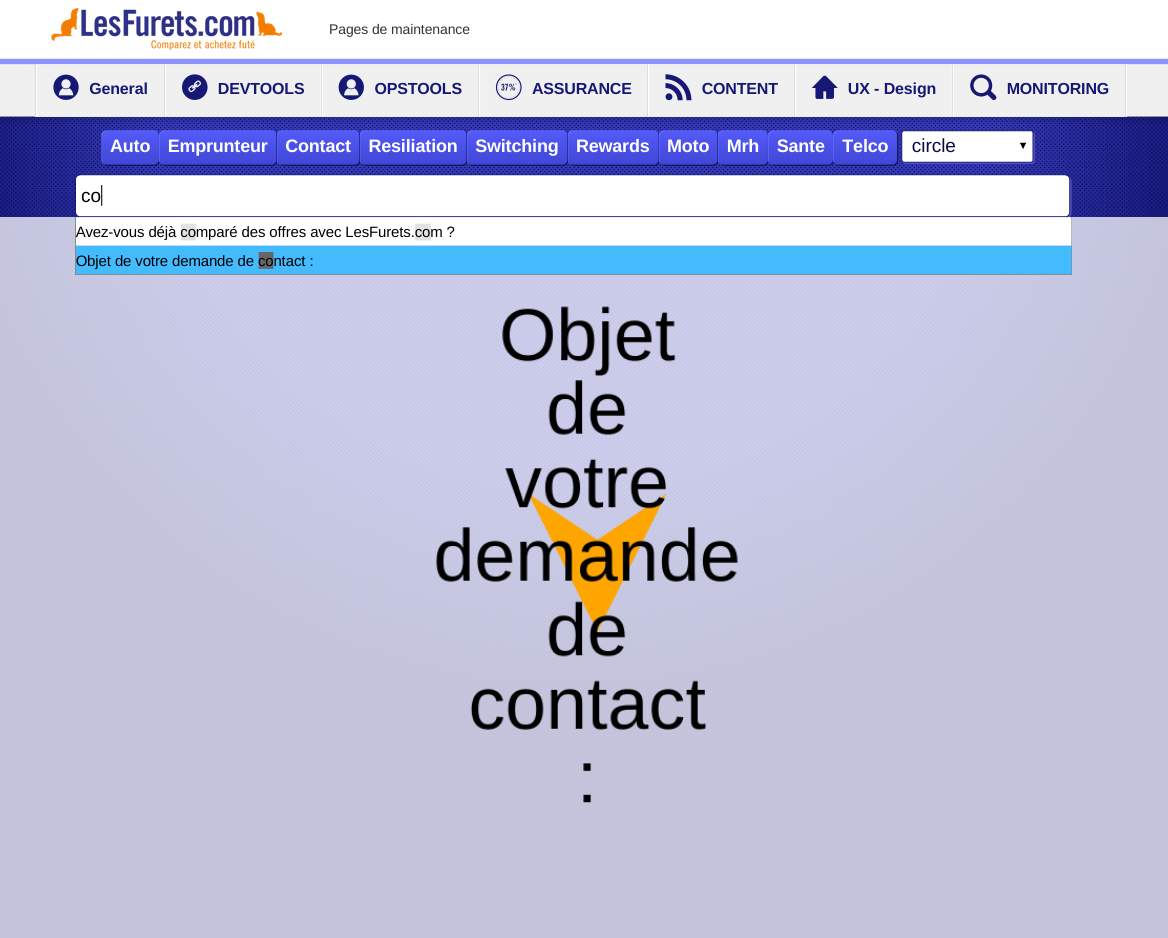
\includegraphics[height=4cm]{outil/feature-search-2.png}
\end{figure}
\subsection{Champs du formulaire}
Un autre gros morceaux du problème était de pouvoir afficher chaque champ dans un style semblable a celui présent dans les formulaires. Après avoir récupéré une liste de tous les types d'éléments dans le formulaire : bouton, textbox, checkbox, boutons radio, liste, date, ... Cette liste était disponible depuis une Enum Java. Ensuite il a fallu dessiner dans la balise canvas des éléments ayant la forme des champs du formulaire.
\vspace{0.5in}
\begin{figure}[!h]
\centering
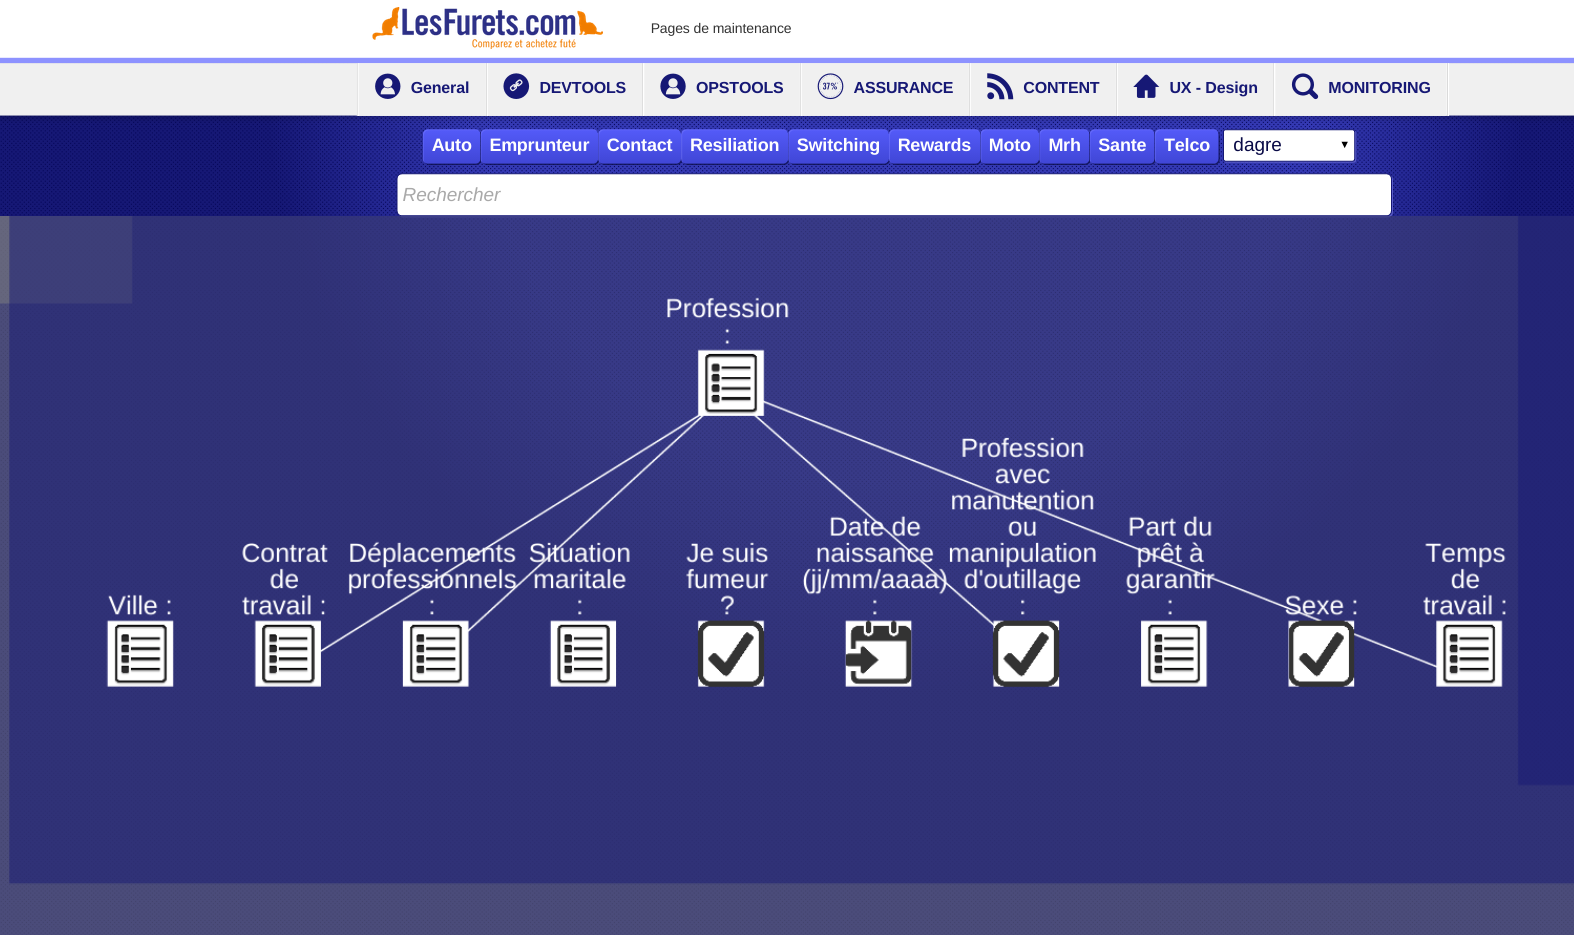
\includegraphics[height=4cm]{outil/layout-field.png}
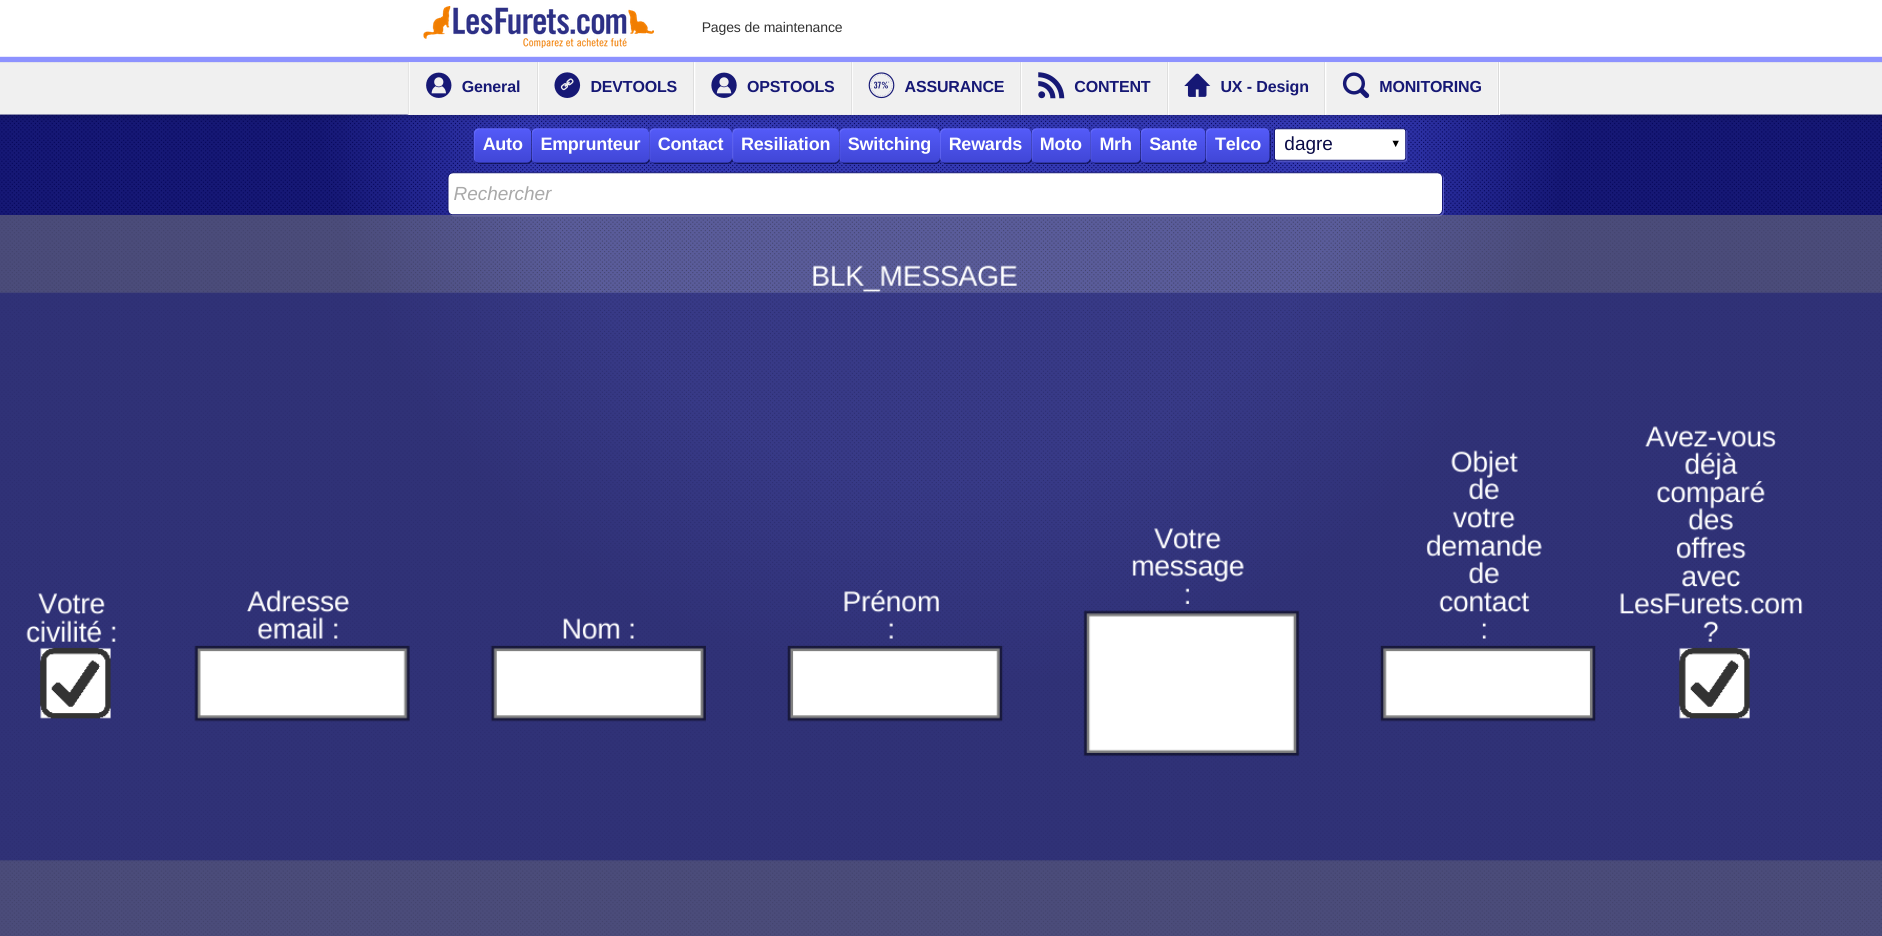
\includegraphics[height=4cm]{outil/layout-field-2.png}
\caption{Différents type de champs du formulaire}
\end{figure}

\clearpage
\subsection{Modification des éléments et des dépendances}
Une fois la phase de "Layout" réalisée il a fallu mettre en place des fonctions de modification/suppression des éléments du graphe. Et une fonction de modifications des dépendances entre les champs.

\subsubsection{Modification du label du champs}
La première fonction était sans doute celle qui avait le moins d’incidence sur le formulaire. Il s'agit de proposer aux utilisateur de pouvoir changer le nom d'un champ du formulaire.

\subsubsection{Modification type du champs}
On proposera aussi à l'utilisateur de pouvoir changer le type d'un champ sélectionné. Pour cela il a fallu lister tous les types de champs disponibles. J'ai pu servir directement dans la JSP la liste des types de champs possibles à l'aide d'une Enum présente dans le code Java.

\subsubsection{Suppression d’une dépendance}
Il s’agit juste de mettre en évidence les champs affectés par la suppression d’une dépendance. Les dépendances ne sont pas interdépendantes. On soulignera les champs impactés par la suppression d'une couleur rouge.
\clearpage
\subsection{Opération sur le graphe}
\subsubsection{Sauvegarde du graphe}
Une fois les fonctions de modifications mise en place il a paru évident qu’il a fallait pouvoir sauvegarder l’état du graphe modifié pour pouvoir l’envoyer par la suite.
La première approche simple était de pouvoir faire une capture d’écran de l’état du graphe dans une résolution assez grande pouvoir voit toute les détails du formulaire.
La seconde approche fut de sauvegarder un fichier JSON avec toutes les données modifié ainsi que les position des champs. En effet Cytoscape accepte de bloquer une position à la création du graphe sous la forme de coordonnée cartésiennes. Il a ensuite fallu définir un repère qui correspondait au repère de base de Cytoscape. Enfin on enregistre la collection d'éléments sous la forme d'un fichier JSON. Une fois le fichier JSON crée on encode une chaîne de caractère en base64 et on crée le fichier 

\subsubsection{Charger un graphe}
Une fois qu'on a donné la possibilité aux utilisateurs de sauvegarder le graphe, il a fallu implémenter un module d’import. A l'aide d'une balise input file, on télécharge le fichier précédemment sauvegarder et on affiche le graphe.

\subsubsection{Calcul des différences}
Une fois le graphe importé nous avons voulu aussi proposer une visualisation des différences entre la version courante et une version importée. Une fois le fichier importé on se retrouver en présence de deux objets JavaScript que l'on peut aisément comparer. Dans le calcul des différences on proposera deux scénario. Le premier est d'afficher graphiquement les différences sur le graphe, à l'aide de couleurs différentes. Le second scénario correspond à servir une liste des différences sous la forme d'une réponse JSON.

\subsubsection{Versionnement du graphe}
En se servant du module de calcul de différences en mode non graphique, l'outil peut versionner un fichier des différences que l'on commitera avec nouvelle version du master. Une future amélioration serait de pouvoir lever une alerte si un trop grand nombre d'objets sont différents.

\clearpage
\section{Données Business}

\subsection{Récupération des données}
Après différentes discussions avec les équipes en charge de la conception de l’application nous avons décidé de ne pas faire des appels à la base SQL à chaque affichage du graphe.
Cependant il m'a été conseillé d'utiliser les données retournées par des batches (Jobs) en charge de récupérer des informations à intervalles réguliers. Les informations fournies par ces batches servent à créer des dashboards réguliers pour les équipes d'analyse. Ainsi Il nous a fallu quand même définir des règles de tri pour créer un agrégat de données pertinent. Nous avons défini le bloc comme grain d'analyse des données, car c'est le plus petit élément où pour passer d'un bloc à l'autre il faut effectuer une action.

\subsection{Affichage des données}
Une fois les données disponibles, il m'a été demandé de les afficher sous la forme d'une jauge en pourcentage en fonction du nombre d'utilisateur passant l'écran suivant à coté du label de chaque bloc. Si la jauge est en dessous des 50\% on affichera aussi la date du champ ou de la dernière dépendance modifié dans le bloc.